\section{Introduction}
Since the introduction of AlexNet, roughly a decade ago, \textit{Convolutional Neural Networks} (CNNs) have played an important role in \textit{Computer Vision} (CV) \citep{krizhevsky2012imagened}. Recently, however, a new type of architecture, called \textit{Vision Transformer} (VT), gained state of the art performance on common learning benchmarks, including the ImageNet dataset\footnote{At the time of writing the VT \texttt{CoCa} is state of the art, according to \url{https://paperswithcode.com/sota/image-classification-on-imagenet}.}.

Exciting as this may be, a plain VT is not likely to become useful in circumstances with limited training data and/or only consumer-grade hardware available for learning. This is due to a limitation inherent to the VT architecture, which will be elaborated on in section \ref{vits}. Consequently, the current paper investigates whether utilizing \textit{Transfer Learning} (TL) capabilities of VTs can help overcome these limitations, and if this allows VTs to become the preferred architecture in the aforementioned circumstances as well.

Before going into more detail, however, some background information is needed. The remainder of this section will first briefly describe CNNs and VTs, and compare them to one another. What follows, is an explanation of TL, and why it might help VTs in circumstances with limited data/compute available. Finally, related work is discussed, and a research question is proposed.

%\begin{figure}[!tbp]
%    \centering
%    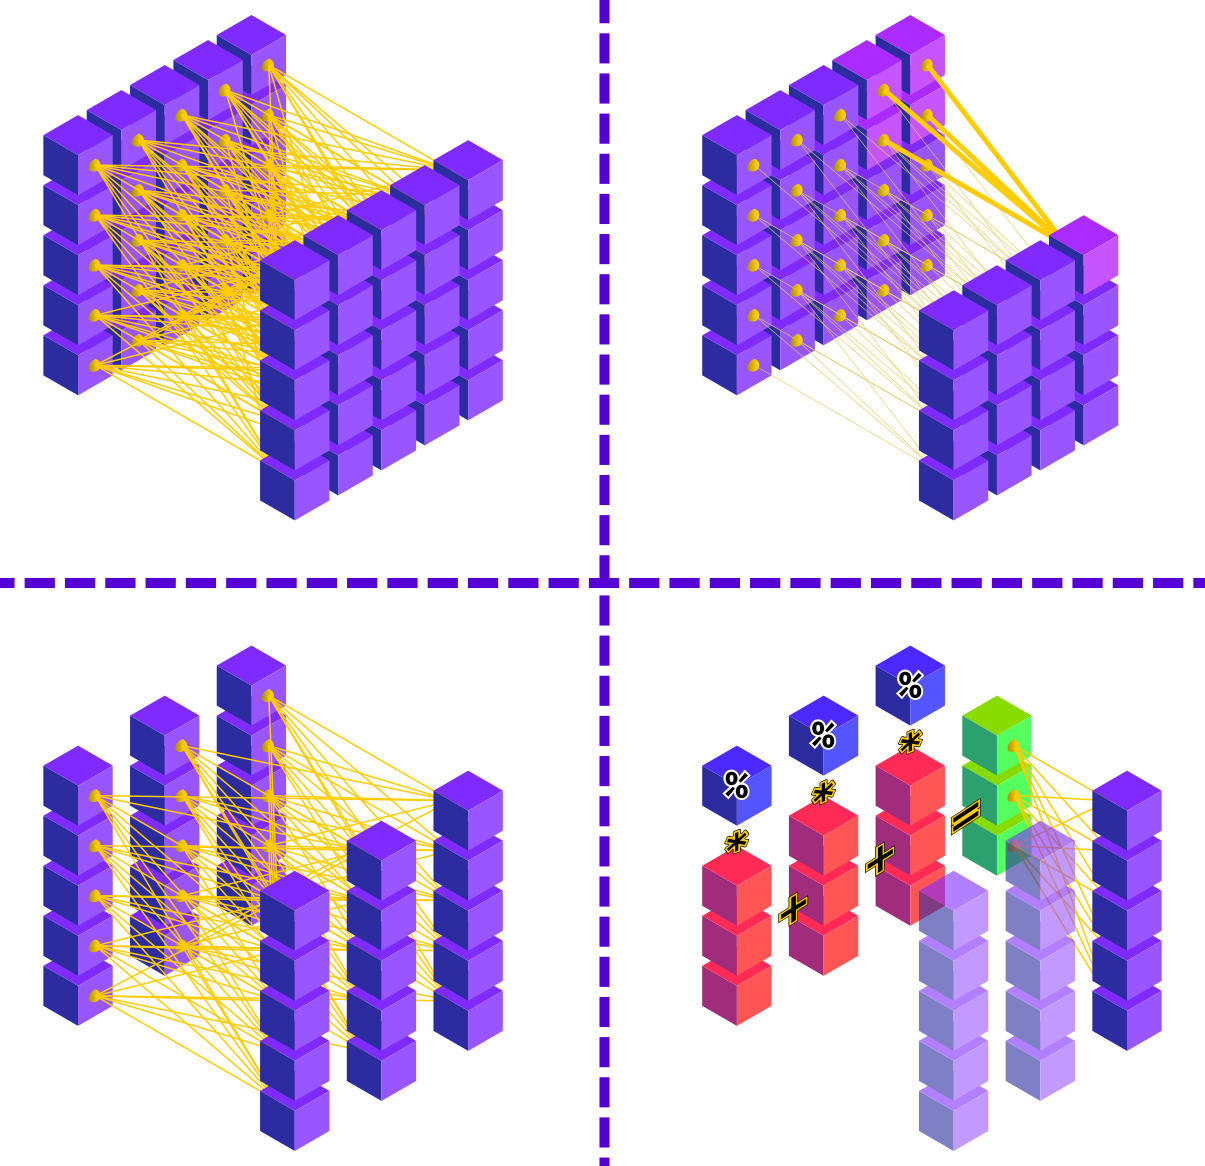
\includegraphics[width=7.7cm]{img/vit_vs_cnn.png}
%    \caption{Intuition behind CNNs and VTs. Note that many details are left out for the purpose of illustration. The top half compares MLP layers (left) to those of CNNs (right). A single neuron and its receptive field are highlighted. Connections are only allowed such as the accentuated 4, which reduces the total number of connections greatly. Moreover, the non-accentuated connections don't add to the number of trainable weights, as the same 4 are shared between all neuron-receptive-field-pairs.\\The bottom half draws a similar comparison between MLPs (left) and VTs (right). A single query vector is combined with all key vectors to get a scalar value for each position (blue boxes). These are multiplied with corresponding value vectors (in red), and then added to get a weighted sum (green). This sum is fed through one or more MLP-type layers, to produce a single output position (opaque). The same steps are taken for all other positions (transparent) as well, using their corresponding query vectors.}
%    \label{vitVsCnn}
%\end{figure}

\subsection{Convolutional Neural Networks}
The modern CNN architecture is often attributed to \citeauthor{lecun1998gradient} (\citeyear{lecun1998gradient}), which describes how the number of trainable weights per layer can be reduced in manners that are sensible for an image's topology (i.e. by restricting connections to a neuron's local receptive field, and by sharing weights).

%which describes how the topology of an image can be taken into account to sensibly reduce the number of weights per layer (i.e. by restricting connections to a neuron's so called local receptive field, and by sharing weights between ).
%The top half of figure \ref{vitVsCnn} attempts to give an intuitive understanding of this, by drawing a comparison to the classical \textit{Multilayer Perceptron} (MLP).

CNNs are largely invariant to shifts and small distortions of the input image. More important, is that they can be seen as automatic feature extractors. It is well established (e.g. \citeauthor{lecun1998gradient}, \citeyear{lecun1998gradient}; \citeauthor{yosinski2014transferable}, \citeyear{yosinski2014transferable}) that the first layers of a CNN detect low level features, such as edges and corners. These are combined in subsequent layers to detect higher order features. The final layer should then give a representative summary of the input, such that, for example, an MLP-type layer can extract all the information it needs from it to perform the task at hand.

%It has asymptotically less trainable parameters per layer than the classical \textit{Multilayer Perceptron} (MLP) [BRON], and achieves this reduction in ways that make sense for the topology of an image. Firstly, connections are restricted to a neuron its so called \textit{local receptive field}. This is a small patch of neurons in the previous layer, with similar spatial location. The top right of figure [FIGREF] shows an example. Here, one neuron and its receptive field are highlighted. The top left shows a hypothetical MLP implementation. Note how it has many more connections overall.

%Secondly, instead of using a different set of trainable weights to connect a neuron to its receptive field, the same set, called a \textit{convolution kernel}, is shared. In figure [FIGREF] the 4 accentuated connections correspond to one such kernel. The other shown connections don't add to the number of trainable weights, as they use this kernel as well. Essentially, a one-layered mini-MLP is slided over the input grid to produce the output grid -- which is called a \textit{feature map}. In reality, multiple kernels and feature maps exist per layer.

%Finally, to reduce the size even further, so called \textit{pooling layers} are added. These reduce the spatial resolution of a feature map by aggregating patches of neurons into one, using $max(\cdot)$, or $mean(\cdot)$, for example.

%\paragraph{Properties}
%The architecture as described, is largely invariant to shifts and small distortions of the input image. More important, is that CNNs can be seen as automatic feature extractors. It is well documented (see, for example, [REFS]) that the first layers of a CNN detect low level features, such as edges and corners. These are combined in subsequent layers to detect higher level features. The final layer then (hopefully) represents the input in an abstract manner, such that, for example, an MLP-type layer can extract all the information it needs from it to perform the task at hand.

\subsection{Vision Transformers} \label{vits}
\paragraph{Architecture}
VTs were first introduced in \citeauthor{dosovitskiy2020image} (\citeyear{dosovitskiy2020image}), and are based on the \textit{encoder stack} of the \textit{Transformer} architecture \citep{vaswani2017attention}. This stack takes a sequence of vectors as input, and is composed of alternating \textit{multi-headed self-attention} layers and position-wise MLP-type layers -- position-wise meaning the MLP can take only a single position (constituent vector) as input at a time, and is shared between all positions.

The self-attention mechanism plays a central role in VTs, and is worth elaborating on. Each head of a self-attention layer contains 3 learned projection matrices, which are used to produce $key$, $value$, and $query$ vectors for every position in the input sequence. The output for a single position is a weighted sum of all $value$ vectors. Weights are obtained by matching this position's $query$ with all $key$ vectors\footnote{In principle by taking softmax over all query-key inner products.}. As such, an attention head decides itself how much of each position should be incorporated in subsequent representations.

The original Transformer architecture was designed to solve problems in \textit{natural language processing} (a field it now dominates). To make it work for CV applications, VTs divide an image into square patches, which get treated as tokens (words). Learned embeddings convert these into a sequence of vectors, to which 1D positional encodings are added\footnote{Do mind that VTs have no built-in knowledge of an image's 2D topology.}. A learned $[class]$ vector gets prepended to the sequence, and its representation at the end of the encoder stack is the final output, which can then be used for classification, segmentation, etc.

%These are converted to learned embeddings, to which 1D position encodings are added. A learned $[class]$ embedding gets prepended to the sequence. 

% TODO Using these it produces weighted sums of value vectors per position. The weights for a position are obtained by combining its $query$ vector with all $key$ vectors\footnote{sofmax TODO}.

%Combining a single $query$ with all keys\footnote{softmax over all dot products. Additionally, all dot products are first divided by the square root of the size of a $key$ vector, as to prevent very small gradients from occurring.}, gives an array of scalars that tells for each $value$ vector how much of it 
% TODO Weight sharing is used in the form of all positions going through the same pipeline

%VTs were first introduced in \citeauthor{dosovitskiy2020image} (\citeyear{dosovitskiy2020image}), and are based on the \textit{Transformer} architecture \citep{vaswani2017attention}. This type of ANN was originally designed to solve problems in \textit{natural language processing} (a field it now dominates). It takes a series of tokens as input, and uses a learned mapping to convert them into a series of vectors, called \textit{token embeddings}. These embeddings are then fed through an encoder and decoder, but since the latter is discarded for VTs, it won't be discussed here.

%, and takes a variable length sequence of \textit{token embeddings}\footnote{The model has some vocabulary of tokens it knows, for example all words in the English language. For each it learns a vector representation, called a token embedding.} as input. While Transformers are made up of an \textit{encoder} and \textit{decoder}, the latter won't be discussed here, as it is discarded in the VT architecture.

%Central to the encoder is the \textit{self-attention mechanism}. The \textit{attention heads} that implement it, start with 3 learned projection matrices.

%The architecture consists of an \textit{encoder}, and \textit{decoder}, but since the latter is discarded in VTs, it won't be discussed here.

%Before entering the encoder, each token is converted into a corresponding vector representation, called a \textit{token embedding}. This is done using a learned mapping from tokens to vectors. To make the network aware of a token's location within the sequence, positional encodings are added to the embeddings as well\footnote{Trigonometric functions are used for this, instead of learned encodings.}.

%The encoder itself is composed of a stack of \textit{encoder blocks}. The first block gets the embeddings as input; the rest the output of its predecessor. Each block contains two components, namely a \textit{multiheaded self-attention} layer, which will be discussed below, and a simple MLP that processes all positions (i.e. vectors) of the input sequence individually. Residual connections add a component's output to its input, and this sum is then normalized; i.e. $Normalize(x + Component(x))$\footnote{Note that this means the dimensions of a component's output are identical to that of its input.}.

%Checklist:
% - constant number of operations to relate tokens, so regardless of distance
% - weight sharing because same learned operations are applied to each (each token goes through the same pipeline)

% While a CNN is restricted to only incorporate information from its surrounding pixels in a subsequent layer, a VT 

\paragraph{CNNs versus VTs}
Where CNNs reduce the number of trainable weights by taking an image's topology into account, VTs do this by learning themselves what information they should incorporate in successive representations of the input. As such, they are not restricted to a local receptive field, but can potentially include information from all over the previous layer.

Moreover, weight sharing applies as much to VTs as it does to CNNs. In VTs, each position goes through the same computational pipelines of being multiplied by 3 projection matrices, followed by a weighted sum calculation, followed by being fed through an MLP-type layer\footnote{Neglecting skip connections and normalization, as this is a comparison on an intuitive level.}. In CNNs these pipelines take the form of convolution kernels.

\paragraph{A limitation of VTs}
While VTs are promising; the fact that they are not tailored to CV tasks, makes that they lack a so called image specific \textit{Inductive Bias}, which CNNs do have. Intuitively this means a VT first has to learn what an image is, before it can move on to the learning task at hand. The result is that they require substantially more training data (and time) than CNNs do. 

It is for this reason the paper that first introduced VTs \citep{dosovitskiy2020image} mentions using pre-trained models rather than randomly initialised ones, as it allows general knowledge about images to be carried over to the new task. This technique falls within the category of TL, which will be covered next.

% CNNs have image specific inductive bias: the architecture itself is tailored to 2D images, and as such has structural information about how images work built-in. This is not the case for VTs, which lack an image specific inductive bias, which makes them very data hungry.

\subsection{Transfer Learning}
Given two \textit{Machine Learning} (ML) problems, of which one is called the source, and the other the target task, Transfer Learning can be defined as \textit{exploiting knowledge implied in the source task to improve performance of an ML model on the target task}. A formal definition is found on p. 56 of \citeauthor{sabatelli2022contributions} (\citeyear{sabatelli2022contributions}), but for the purposes of this paper, the one above suffices.

In practice, many TL techniques exist. The example given in section \ref{vits} can be described as \textit{fine-tuning} (FT) TL. Here, a pre-trained model is used as a starting point, and then trained on the target task -- possibly with different hyperparameters, and often with a new final layer that fits the task. \citeauthor{yosinski2014transferable} (\citeyear{yosinski2014transferable}) studied transferability properties of CNNs pre-trained on ImageNet, and suggested that FT results in improved performance and generalizability compared to training from scratch. Moreover, while transferability decreased as source and target task became more dissimilar, utilizing TL still seemed to be preferred.

% FINE-TUNING: "yosinski2014transferable" CNNs
% 1) Lower layers contain general information that can easily be transferred (deze doe ik naar volgende stukje misschien)
% 2) Distance between source and target task increases -> transferability decreases
%       - BUT: still better than randomly initialized
% 3) Increases generalizability (This one is important for me ;-) )

A different TL technique is called \textit{off-the-shelf} (OTS) TL. It is similar to FT, except that all but the final layer is kept frozen during training. \citeauthor{sharif2014cnn} (\citeyear{sharif2014cnn}) found that features extracted by a CNN pre-trained on ImageNet were general enough for OTS TL to work. More specifically, these OTS CNNs showed better performance than the (fully trained non-CNN) state of the art at the time. Besides reducing computational cost of training, a benefit of OTS TL is that it can prevent overfitting in cases where FT would not \citep{yosinski2014transferable}.

% TODO!!! Maybe mention TL is a solution when target dataset is much smaller, and maybe mention model TL technique: information passed between source and target in the form of a pre-trained model!!! TODO TODO TODO
% OFF-THE-SHELF:
% 1) "yosinski2014transferable": OTS can prevent overfitting where fine-tuning would overfit
% 2) "yosinski2014transferable": first layers general information

\subsection{Related work and the current study} \label{related_work}
As mentioned, the paper that first introduced VTs already demonstrated they benefit from TL \citep{dosovitskiy2020image}, and more has been discovered about VTs' TL properties since then. \citeauthor{matsoukas2021time} (\citeyear{matsoukas2021time}) investigated whether TL allowed VTs to replace CNNs in Medical Imaging. This domain is characterized by small datasets, so to overcome the inductive bias problem described earlier, TL is imperative. It was found that VTs benefit more from FT TL than CNNs do, and that VTs pre-trained on ImageNet perform on par CNNs.

What \citeauthor{matsoukas2021time} did not investigate, is OTS performance of VTs. This was, however, done in \citeauthor{zhou2021convnets} (\citeyear{zhou2021convnets}), which found that VTs pre-trained on ImageNet had worse OTS performance than their CNN counterparts. An exception was the \texttt{Swin} architecture, which was the best performing model on all datasets, and uses \textit{(shifted-)window-based} self-attention methods, to make Transformers better suited for CV tasks \citep{liu2021swin}.
% Not into detail about ots and other techniques

Another ``shortcomming'' of \citeauthor{matsoukas2021time} is that it merely examined whether VTs can use TL to outperform CNNs in a domain that happens to be characterized by limited-sized datasets, but that it did not actively focus on the extent to which VTs can be made useful in limited data/compute environments. More related to this is \citeauthor{touvron2021training} (\citeyear{touvron2021training}), which proposed transformer-specific distillation-based learning techniques to make VTs applicable for smaller datasets. This is not necessarily related to TL as defined in this paper, however.
% matsoukas2021time not specifically focussed on seeing to what degree TL allows VTs to dominate CNNs in limited compute/data environments
\\\\
The current study will examine to what extent TL techniques (both FT and OTS) allow VTs to become the preferred architecture when compute resources are limited, and attempts to find a methodology that is recommended in these circumstances. It will, however, restrict itself to art classification tasks. Several experiments will be performed, of which results will be analysed both quantitatively as well as qualitatively.

%TODO: talk about datasets small enough to be hand labelled by one person
%The current study limits itself to the task of identifying which materials were used in artworks. For this, it will examine to what extent TL techniques (both fine-tuning and OTS) allow VTs to become the preferred architecture when compute resources are limited, and attempt to find a methodology that is preferred in circumstances as described. It will do this by means of several experiments, and both quantitative and qualitative analysis of the results.

More formally, the following research question is proposed: \begin{quote}\textit{To what extent (and in what manners) does utilizing TL allow VTs to perform on par with CNNs on common art classification problems, when compute resources are limited to a single GPU?}\end{quote}
